\begin{figure*}
\centering
\begin{tikzpicture}
[ p/.style={ draw=none, fill=none, }, remember picture, 
  net/.style={ matrix of nodes, nodes={ draw, circle, inner sep=7.5pt },
  nodes in empty cells,
  column sep=-10.5pt,
  row sep=0.8cm
  }
]
%\draw[help lines] (-3cm,-6cm) grid (6cm,3cm);
\matrix[net] (mat)
{
	  & |[p]| &  & |[p]| &  & |[p]| &  & |[p]| &  & |[p]| &  & |[p]| &  & |[p]| &  & |[p]| &  &
	    |[p]| &  & |[p]| &  & |[p]| &  & |[p]| &  & |[p]| &  & |[p]| &  & |[p]| &  & |[p]|    \\
 |[p]| & |[p]| & |[p]| &  |[p]| &        & |[p]| & |[p]| & |[p]| &|[p]| &       & |[p]| &  |[p]| & |[p]| &
 |[p]| &       & |[p]| &  |[p]| &  |[p]| & |[p]| & |[p]| &       &|[p]| & |[p]| & |[p]| & |[p]|
	   & |[p]| &       &  |[p]| &  |[p]| & |[p]| & |[p]| & |[p]| &|[p]| \\ 
 |[p]| &  |[p]| & |[p]|  &  |[p]| & |[p]|  &  |[p]| &  |[p]| &  |[p]| & |[p]| & |[p]| & |[p]| &       & |[p]|
	   &  |[p]| & |[p]|  &  |[p]| &        &  |[p]| &  |[p]| &  |[p]| & |[p]| & |[p]| & |[p]| & |[p]| &     |[p]|
	   &  |[p]| & |[p]|  &  |[p]| & |[p]|  &  |[p]| &  |[p]| &  |[p]| \\ 
  };
  \draw[<-] (mat-1-1.north) --  ++(0,1) node {$N_x$};
  \draw[<-] (mat-1-3.north) --  ++(0,1) node {$N_y$};
  \draw[<-] (mat-1-5.north) --  ++(0,1) node {$N_{xy}$};
  \draw[<-] (mat-1-7.north) --  ++(0,1) node {$\theta_1$};
  \draw[<-] (mat-1-9.north) --  ++(0,1) node {$\theta_2$};
  \draw[<-] (mat-1-11.north) --  ++(0,1) node {$t$};
  \draw[<-] (mat-1-13.north) --  ++(0,1) node {$N$};
  \draw[<-] (mat-1-15.north) --  ++(0,1) node {$E_1$};
  \draw[<-] (mat-1-17.north) --  ++(0,1) node {$E_2$};
  \draw[<-] (mat-1-19.north) --  ++(0,1) node {$G_{12}$};
  \draw[<-] (mat-1-21.north) --  ++(0,1) node {$v_{12}$};
  \draw[<-] (mat-1-23.north) --  ++(0,1) node {$\sigma_1^T$};
  \draw[<-] (mat-1-25.north) --  ++(0,1) node {$\sigma_1^C$};
  \draw[<-] (mat-1-27.north) --  ++(0,1) node {$\sigma_2^T$};
  \draw[<-] (mat-1-29.north) --  ++(0,1) node {$\sigma_2^C$};
  \draw[<-] (mat-1-31.north) --  ++(0,1) node {$\tau_{12}$};
  \draw[->] (mat-3-12.south) --  ++(0,-1) node[pos=0.5, swap] {Tsai-Wu};
  \draw[->] (mat-3-17.south) --  ++(0,-1) node[pos=0.5, swap] {MS};
  \node at ($(mat-1-1.west)+(-16pt,0)$) {Input: };
  \node at ($(mat-2-2.west)+(-24pt,0)$) {Hidden:};
  \node at ($(mat-3-2.west)+(-24pt,0)$) {Output:};
  \node at (mat-2-5.base) {$h_1$};
  \node at (mat-2-10.base) {$h_2$};
  \node at (mat-2-15.base) {$...$};
  \node at (mat-2-21.base) {\small{$h_{m-1}$}};
  \node at (mat-2-27.base) {$h_{m}$};
 \foreach \a in {1,3,5,7,9,11,31}{
        \draw[->] (mat-1-\a.south) -- (mat-2-5.north);
     }
 \foreach \a in {5,7,11,19,25,27}{
        \draw[->] (mat-1-\a.south) -- (mat-2-10.north);
     }
 \foreach \a in {1,7,11,17,19,25}{
        \draw[->] (mat-1-\a.south) -- (mat-2-15.north);
     }
 \foreach \a in {5,9,19,21,29}{
        \draw[->] (mat-1-\a.south) -- (mat-2-21.north);
     }
 \foreach \a in {11,15,19,23,27,29,31}{
        \draw[->] (mat-1-\a.south) -- (mat-2-27.north);
     }
 \foreach \c in {5,10,15,21,27}{
    \foreach \d in {12,17}{
 		\draw[->] (mat-2-\c.south) -- (mat-3-\d.north);
	}
 }
\end{tikzpicture}
\caption{Neural Network Model}
\end{figure*}

The inputs of the neural network is consist of four parts: in-plane loading
$N_x$, $N_y$, and $N_{xy}$, design parameters of laminate, two distinct fiber
orientation angle $\theta_1$ and $\theta_2$, ply thickness $t$, total number of
plies $N$; five engineering constants of composite materials, $E_1$, $E_2$, ;
five strength parameters of a unidirectional lamina. There are two outputs in
the neural network, safety factors for MS theory and Tsai-Wu theory, respectively.

\begin{figure}
\centering
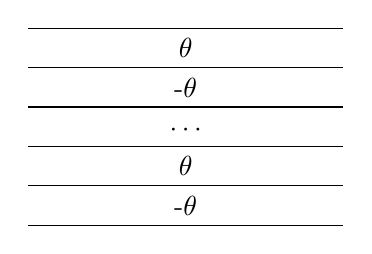
\begin{tikzpicture}
	\draw (0,0) -- (4,0);
	\draw (0,-0.5) -- (4,-0.5) node[midway, above] {$\theta$};
	\draw (0,-1) -- (4,-1) node[midway, above] {\text{-}$\theta$};
	\draw (0,-1.5) -- (4,-1.5) node[midway, above] {$\cdots$};
	\draw (0,-2) -- (4,-2) node[midway, above] {$\theta$};
	\draw (0,-2.5) -- (4,-2.5) node[midway, above] {\text{-}$\theta$};
\end{tikzpicture}
\caption{Model for Angle ply laminate}
\end{figure}

